\subsection{The \acs{OLS} Assumptions Verification}
\label{appendix: assumptions}

In this appendix, we show whether the extended least squares assumptions (\ie\,\acs{CLM} assumptions) are satisfied in our model. If \ref{appendix:zero_cond_assump} to \ref{appendix:outliers} are satisfied, by \acs{GMT}, the \acs{OLS} estimator is \acs{BLUE} and \acs{MVUE} \cite{stock_watson_2019, wooldridge_2020}. However, in practice, the economic applications are often heteroscedastic, but that does not mean the estimators are less efficient than \acs{OLS} \cite{christopher_2006, stock_watson_2019}. \ref{appendix:normality} is not required for asymptotic analysis \cite{wooldridge_2020}.

\subsubsection{$\epsilon_{i}$ has conditional mean zero}\label{appendix:zero_cond_assump}
Equivalently, the expectation of the stochastic error term $\epsilon$ is zero given all values of the independent variables. Mathematically speaking, we have
\begin{equation} \label{eq:zero_cond_assump}
\mathop{\mathbb{E}}[\,\epsilon \mid X_{1i},\dots,X_{ki}\,]=0
\end{equation}

To verify Equation (\ref{eq:zero_cond_assump}), we check whether our model has functional form misspecification, \acs{OVB}, measurement error in an explanatory variable \cite{wooldridge_2020}. These tests are sufficient, but not necessary conditions to prove the assumption \cite{studenmund_2017}. We use Ramsey's \acs{RESET} as a general test for functional form misspecification, and it has been proven to be useful and can be made robust to heteroskedasticity \cite{christopher_2006, wooldridge_2020, studenmund_2017}. In our model, though \acs{RESET} was rejected, we built our model based on economic literature and intuition, and thus we believe our model provides satisfactory interpretations in \hyperref[sec:results]{\text{Results}}. For \acs{OVB}, our multiple regression analysis has a lower probability of \acs{OVB} compared to single regression analysis \cite{wooldridge_2020}. Also, adding one or more regressors not necessarily affects the adequacy of the model, observed from Table \ref{tab:regression}. Therefore, in our case, we included the hidden biases and measurement error in the stochastic error term $\epsilon$ \cite{studenmund_2017}.

\subsubsection{$(X_{1i}$, $X_{2i}$,\dots, $X_{ki}$, $Y_{i})\,$ are \acs{i.i.d} drawn from their joint distribution}
We check this assumption by considering if the data are collected by simple random sampling \cite{stock_watson_2019}. In our case, it is very plausible to have this assumption based on \acs{CPS}'s sampling designs and techniques. Moreover, an important feature of cross-sectional data is that we can assume the samples are randomly selected from the population \cite{wooldridge_2020}.

\subsubsection{No perfect multicollinearity}
To show no perfect multicollinearity between predictor variables, we show that the matrix $\pmb{X}^T\pmb{X}$ is nonsingular\footnote{A matrix is nonsingular is equivalent to that a matrix is invertible or a matrix has full rank.} so that the solution of $\pmb{\hat{\beta}}$ is unique in Equation (\ref{eq:ols_sol3}) \cite{christopher_2006, stock_watson_2019, kuter_nachtsheim_neter_li_2005}. We verified the matrix is nonsingular using Stata in our regression results\footnote{Invertible matrix theorems and properties help us to determine multicollinearity by hand.}.

For imperfect multicollinearity, we check by calculating the \hyperref[appendix:notations]{\text{VIFs}} of the variables. The results are shown in Table \ref{tab:vif}. As a rule of thumb, we are able to conclude that there is high collinearity between the explanatory variable and explained variables when the largest \hyperref[appendix:notations]{\text{VIF}} is bigger than 10 \cite{christopher_2006, kuter_nachtsheim_neter_li_2005, wooldridge_2020}. Yet, the \hyperref[appendix:notations]{\text{VIFs}} test is a sufficient but not a necessary condition to conclude multicollinearity \cite{studenmund_2017}.

\begin{table}
\makebox[\textwidth][c]{
\begin{tabular}{l*{1}{|ccc}}

Variable    &         VIF&       1/VIF&\\
\hline
Nonmarried  &        1.31&        0.76&\\
Age         &        1.30&        0.77&\\
Education   &        1.05&        0.96&\\
US          &        1.03&        0.97&\\
Male        &        1.02&        0.98&\\
\hline
Mean VIF    &        1.14&            &\\

\end{tabular}
}
\caption{\label{tab:vif}
\textit{estat vif}\protect\footnotemark for explanatory variables}
\end{table}

\footnotetext{\textit{estat vif} is a Stata command used to find \hyperref[appendix:notations]{\text{VIFs}} for the independent variables.}




\subsubsection{Homoskedasticity}\label{appendix:homoskedasticity}
Homoskedasticity means that the error term $\epsilon$ has a finite constant variance. \ie 
\begin{equation} \label{eq:homoskedasticity}
\mathrm{Var}[\,\epsilon \mid X_{1i},\dots,X_{ki}\,]= \sigma^2 < \infty
\end{equation}
We check homoskedasticity by graphing the fitted values and residuals, shown in Figure \ref{fig:rvfplot}. It is not reasonable to assume homoskedasticity since more and more residuals of data points are negative towards the right tail, which indicates a sign of heteroscedasticity \cite{studenmund_2017}. Or, we use Cameron \& Trivedi's decomposition of IM-test to see whether the null hypothesis, the variance of the residuals is constant, can be rejected. The result is shown in Table \ref{tab:im}. Thus, we have sufficient evidence to say that our OLS estimator is heteroskedastic. Heteroskedasticity typically causes \acs{OLS} to no longer be an \acs{MVUE} \cite{studenmund_2017}.

\begin{table}
\makebox[\textwidth][c]{
\begin{tabular}{l*{1}{|cccc}}

Source            &        chi2&          df&           p&\\
\hline
Heteroskedasticity&     1504.45&          31&        0.00&\\
Skewness          &     3952.01&           8&        0.00&\\
Kurtosis          &      222.82&           1&        0.00&\\
\hline
Total             &     5679.28&          40&        0.00&\\

\end{tabular}
}
\caption{\label{tab:im}
\textit{estat imtest}\protect\footnotemark for heteroskedasticity, skewness and kurtosis}
\end{table}

\footnotetext{\textit{estat imtest} is a Stata command used to perform an information matrix test for the regression model and an orthogonal decomposition into tests for heteroskedasticity, skewness, and kurtosis due to Cameron and Trivedi (1990).}

\begin{figure}[ht]
  \centering
  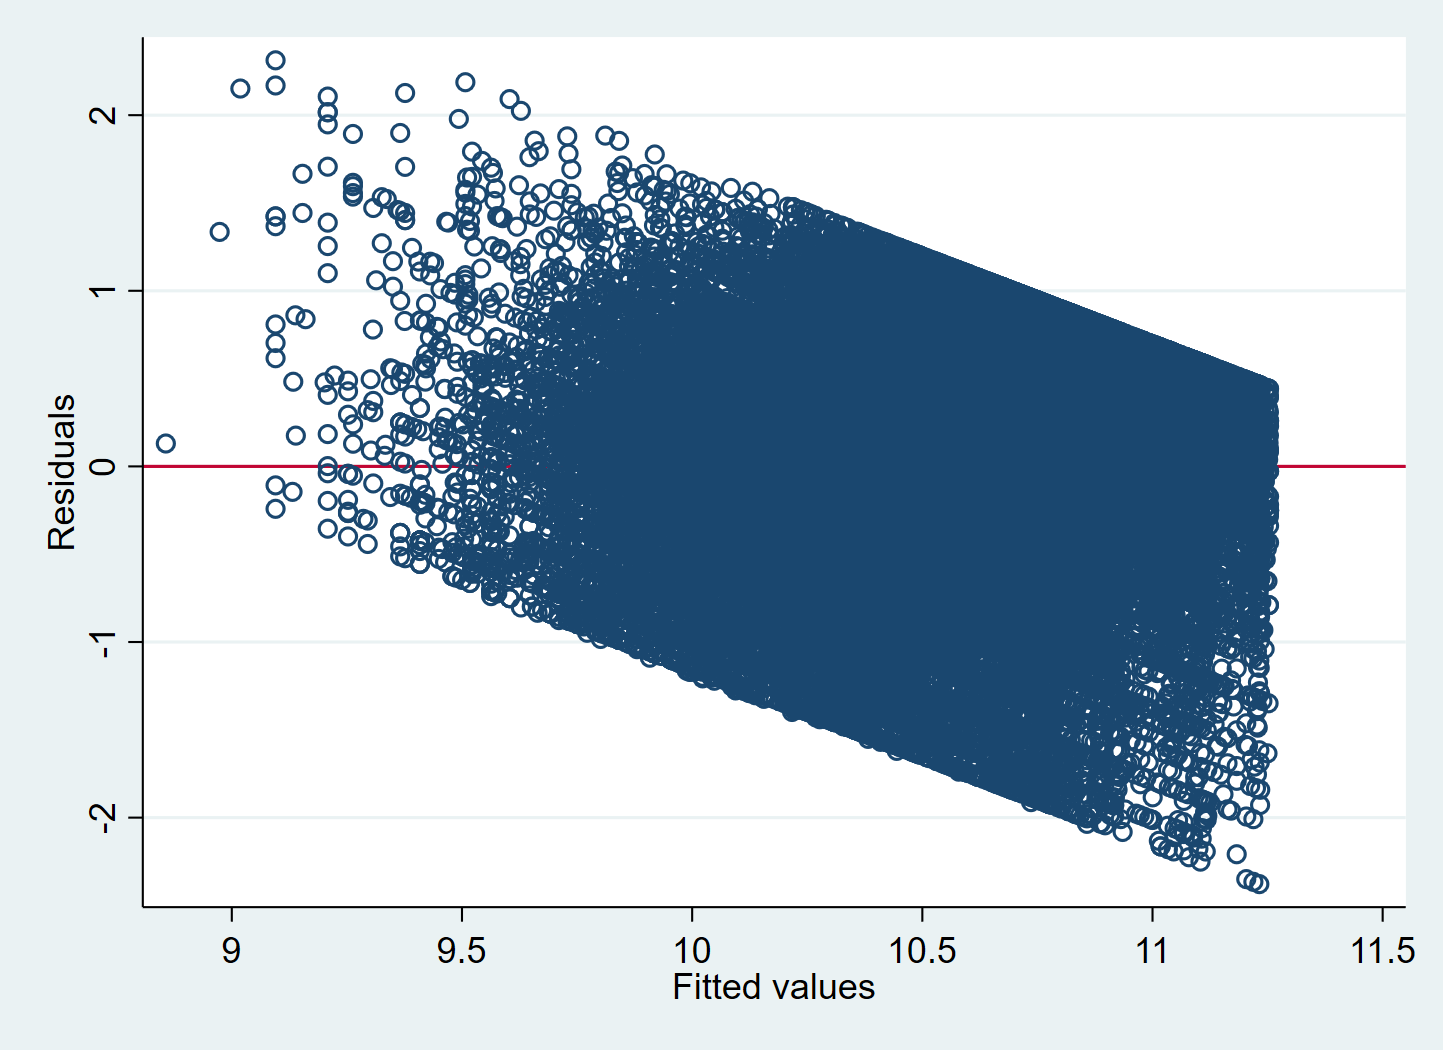
\includegraphics[scale=0.2]{{figures/graph_rvfplot}}
  \caption{\label{fig:rvfplot}
  \textit{rvfplot}\protect\footnotemark of fitted values and residuals
   }
\end{figure}

\footnotetext{\textit{rvfplot} is a Stata command used to graph a residual-versus-fitted plot, a graph of the residuals against the fitted values.}



\subsubsection{Large outliers are unlikely}\label{appendix:outliers}
Mathematically speaking, we say that it is unlikely to have large outliers if
\[
0<\mathop{\mathbb{E}}[\,X_{1i}^4\,]<\infty \quad \eqcomma \dotsm \eqcomma \quad 0<\mathop{\mathbb{E}}[\,X_{ki}^4\,]<\infty\eqcomma \quad and \quad 0<\mathop{\mathbb{E}}[\,Y_{i}^4\,]<\infty
\]
We already cleaned our data set by using Box-and-Whisker plots as mentioned in \hyperref[sec:data]{\text{Data}} section. Another way to state this assumption is that $X$ and $Y$ have finite kurtosis \cite{stock_watson_2019}. We found that all variables have a finite kurtosis using Stata, though we reject the hypothesis that the kurtosis is normal (See Table \ref{tab:im}).

\subsubsection{Normal errors}\label{appendix:normality}
Normal errors refer to the normality of our error term $\epsilon$:
\[
\epsilon \sim \mathcal{N}(0,\,\sigma^{2})
\]
In multivariate regression, \acs{CLT} applies to the \acs{OLS} estimators as well \cite{christopher_2006, stock_watson_2019}. \ie\,$\hat{\beta_{i}} \sim \mathcal{N}(\beta_{i},\,\sigma^{2}_{\hat{\beta_{i}}})$. In our case, since the model is heteroscedastic, it is hard to conclude that the errors are normal \cite{wooldridge_2020}. However, we can observe the error follows asymptotic normality in some extent in Figure (\ref{fig:rvfplot}). When sample size is large, the distributions of the regression coefficients approach normality under general conditions \cite{kuter_nachtsheim_neter_li_2005}.